
%% bare_conf.tex
%% V1.4a
%% 2014/09/17
%% by Michael Shell
%% See:
%% http://www.michaelshell.org/
%% for current contact information.
%%
%% This is a skeleton file demonstrating the use of IEEEtran.cls
%% (requires IEEEtran.cls version 1.8a or later) with an IEEE
%% conference paper.
%%
%% Support sites:
%% http://www.michaelshell.org/tex/ieeetran/
%% http://www.ctan.org/tex-archive/macros/latex/contrib/IEEEtran/
%% and
%% http://www.ieee.org/

%%*************************************************************************
%% Legal Notice:
%% This code is offered as-is without any warranty either expressed or
%% implied; without even the implied warranty of MERCHANTABILITY or
%% FITNESS FOR A PARTICULAR PURPOSE! 
%% User assumes all risk.
%% In no event shall IEEE or any contributor to this code be liable for
%% any damages or losses, including, but not limited to, incidental,
%% consequential, or any other damages, resulting from the use or misuse
%% of any information contained here.
%%
%% All comments are the opinions of their respective authors and are not
%% necessarily endorsed by the IEEE.
%%
%% This work is distributed under the LaTeX Project Public License (LPPL)
%% ( http://www.latex-project.org/ ) version 1.3, and may be freely used,
%% distributed and modified. A copy of the LPPL, version 1.3, is included
%% in the base LaTeX documentation of all distributions of LaTeX released
%% 2003/12/01 or later.
%% Retain all contribution notices and credits.
%% ** Modified files should be clearly indicated as such, including  **
%% ** renaming them and changing author support contact information. **
%%
%% File list of work: IEEEtran.cls, IEEEtran_HOWTO.pdf, bare_adv.tex,
%%                    bare_conf.tex, bare_jrnl.tex, bare_conf_compsoc.tex,
%%                    bare_jrnl_compsoc.tex, bare_jrnl_transmag.tex
%%*************************************************************************


% *** Authors should verify (and, if needed, correct) their LaTeX system  ***
% *** with the testflow diagnostic prior to trusting their LaTeX platform ***
% *** with production work. IEEE's font choices and paper sizes can       ***
% *** trigger bugs that do not appear when using other class files.       ***                          ***
% The testflow support page is at:
% http://www.michaelshell.org/tex/testflow/



\documentclass[journal]{IEEEtran}
% Some Computer Society conferences also require the compsoc mode option,
% but others use the standard conference format.
%
% If IEEEtran.cls has not been installed into the LaTeX system files,
% manually specify the path to it like:
% \documentclass[conference]{../sty/IEEEtran}





% Some very useful LaTeX packages include:
% (uncomment the ones you want to load)


% *** MISC UTILITY PACKAGES ***
%
%\usepackage{ifpdf}
% Heiko Oberdiek's ifpdf.sty is very useful if you need conditional
% compilation based on whether the output is pdf or dvi.
% usage:
% \ifpdf
%   % pdf code
% \else
%   % dvi code
% \fi
% The latest version of ifpdf.sty can be obtained from:
% http://www.ctan.org/tex-archive/macros/latex/contrib/oberdiek/
% Also, note that IEEEtran.cls V1.7 and later provides a builtin
% \ifCLASSINFOpdf conditional that works the same way.
% When switching from latex to pdflatex and vice-versa, the compiler may
% have to be run twice to clear warning/error messages.






% *** CITATION PACKAGES ***
%
%\usepackage{cite}
% cite.sty was written by Donald Arseneau
% V1.6 and later of IEEEtran pre-defines the format of the cite.sty package
% \cite{} output to follow that of IEEE. Loading the cite package will
% result in citation numbers being automatically sorted and properly
% "compressed/ranged". e.g., [1], [9], [2], [7], [5], [6] without using
% cite.sty will become [1], [2], [5]--[7], [9] using cite.sty. cite.sty's
% \cite will automatically add leading space, if needed. Use cite.sty's
% noadjust option (cite.sty V3.8 and later) if you want to turn this off
% such as if a citation ever needs to be enclosed in parenthesis.
% cite.sty is already installed on most LaTeX systems. Be sure and use
% version 5.0 (2009-03-20) and later if using hyperref.sty.
% The latest version can be obtained at:
% http://www.ctan.org/tex-archive/macros/latex/contrib/cite/
% The documentation is contained in the cite.sty file itself.






% *** GRAPHICS RELATED PACKAGES ***
%
\ifCLASSINFOpdf
  % \usepackage[pdftex]{graphicx}
  % declare the path(s) where your graphic files are
  % \graphicspath{{../pdf/}{../jpeg/}}
  % and their extensions so you won't have to specify these with
  % every instance of \includegraphics
  % \DeclareGraphicsExtensions{.pdf,.jpeg,.png}
\else
  % or other class option (dvipsone, dvipdf, if not using dvips). graphicx
  % will default to the driver specified in the system graphics.cfg if no
  % driver is specified.
  % \usepackage[dvips]{graphicx}
  % declare the path(s) where your graphic files are
  % \graphicspath{{../eps/}}
  % and their extensions so you won't have to specify these with
  % every instance of \includegraphics
  % \DeclareGraphicsExtensions{.eps}
\fi
% graphicx was written by David Carlisle and Sebastian Rahtz. It is
% required if you want graphics, photos, etc. graphicx.sty is already
% installed on most LaTeX systems. The latest version and documentation
% can be obtained at: 
% http://www.ctan.org/tex-archive/macros/latex/required/graphics/
% Another good source of documentation is "Using Imported Graphics in
% LaTeX2e" by Keith Reckdahl which can be found at:
% http://www.ctan.org/tex-archive/info/epslatex/
%
% latex, and pdflatex in dvi mode, support graphics in encapsulated
% postscript (.eps) format. pdflatex in pdf mode supports graphics
% in .pdf, .jpeg, .png and .mps (metapost) formats. Users should ensure
% that all non-photo figures use a vector format (.eps, .pdf, .mps) and
% not a bitmapped formats (.jpeg, .png). IEEE frowns on bitmapped formats
% which can result in "jaggedy"/blurry rendering of lines and letters as
% well as large increases in file sizes.
%
% You can find documentation about the pdfTeX application at:
% http://www.tug.org/applications/pdftex





% *** MATH PACKAGES ***
%
%\usepackage[cmex10]{amsmath}
% A popular package from the American Mathematical Society that provides
% many useful and powerful commands for dealing with mathematics. If using
% it, be sure to load this package with the cmex10 option to ensure that
% only type 1 fonts will utilized at all point sizes. Without this option,
% it is possible that some math symbols, particularly those within
% footnotes, will be rendered in bitmap form which will result in a
% document that can not be IEEE Xplore compliant!
%
% Also, note that the amsmath package sets \interdisplaylinepenalty to 10000
% thus preventing page breaks from occurring within multiline equations. Use:
%\interdisplaylinepenalty=2500
% after loading amsmath to restore such page breaks as IEEEtran.cls normally
% does. amsmath.sty is already installed on most LaTeX systems. The latest
% version and documentation can be obtained at:
% http://www.ctan.org/tex-archive/macros/latex/required/amslatex/math/





% *** SPECIALIZED LIST PACKAGES ***
%
%\usepackage{algorithmic}
% algorithmic.sty was written by Peter Williams and Rogerio Brito.
% This package provides an algorithmic environment fo describing algorithms.
% You can use the algorithmic environment in-text or within a figure
% environment to provide for a floating algorithm. Do NOT use the algorithm
% floating environment provided by algorithm.sty (by the same authors) or
% algorithm2e.sty (by Christophe Fiorio) as IEEE does not use dedicated
% algorithm float types and packages that provide these will not provide
% correct IEEE style captions. The latest version and documentation of
% algorithmic.sty can be obtained at:
% http://www.ctan.org/tex-archive/macros/latex/contrib/algorithms/
% There is also a support site at:
% http://algorithms.berlios.de/index.html
% Also of interest may be the (relatively newer and more customizable)
% algorithmicx.sty package by Szasz Janos:
% http://www.ctan.org/tex-archive/macros/latex/contrib/algorithmicx/




% *** ALIGNMENT PACKAGES ***
%
%\usepackage{array}
% Frank Mittelbach's and David Carlisle's array.sty patches and improves
% the standard LaTeX2e array and tabular environments to provide better
% appearance and additional user controls. As the default LaTeX2e table
% generation code is lacking to the point of almost being broken with
% respect to the quality of the end results, all users are strongly
% advised to use an enhanced (at the very least that provided by array.sty)
% set of table tools. array.sty is already installed on most systems. The
% latest version and documentation can be obtained at:
% http://www.ctan.org/tex-archive/macros/latex/required/tools/


% IEEEtran contains the IEEEeqnarray family of commands that can be used to
% generate multiline equations as well as matrices, tables, etc., of high
% quality.




% *** SUBFIGURE PACKAGES ***
%\ifCLASSOPTIONcompsoc
%  \usepackage[caption=false,font=normalsize,labelfont=sf,textfont=sf]{subfig}
%\else
%  \usepackage[caption=false,font=footnotesize]{subfig}
%\fi
% subfig.sty, written by Steven Douglas Cochran, is the modern replacement
% for subfigure.sty, the latter of which is no longer maintained and is
% incompatible with some LaTeX packages including fixltx2e. However,
% subfig.sty requires and automatically loads Axel Sommerfeldt's caption.sty
% which will override IEEEtran.cls' handling of captions and this will result
% in non-IEEE style figure/table captions. To prevent this problem, be sure
% and invoke subfig.sty's "caption=false" package option (available since
% subfig.sty version 1.3, 2005/06/28) as this is will preserve IEEEtran.cls
% handling of captions.
% Note that the Computer Society format requires a larger sans serif font
% than the serif footnote size font used in traditional IEEE formatting
% and thus the need to invoke different subfig.sty package options depending
% on whether compsoc mode has been enabled.
%
% The latest version and documentation of subfig.sty can be obtained at:
% http://www.ctan.org/tex-archive/macros/latex/contrib/subfig/




% *** FLOAT PACKAGES ***
%
%\usepackage{fixltx2e}
% fixltx2e, the successor to the earlier fix2col.sty, was written by
% Frank Mittelbach and David Carlisle. This package corrects a few problems
% in the LaTeX2e kernel, the most notable of which is that in current
% LaTeX2e releases, the ordering of single and double column floats is not
% guaranteed to be preserved. Thus, an unpatched LaTeX2e can allow a
% single column figure to be placed prior to an earlier double column
% figure. The latest version and documentation can be found at:
% http://www.ctan.org/tex-archive/macros/latex/base/


%\usepackage{stfloats}
% stfloats.sty was written by Sigitas Tolusis. This package gives LaTeX2e
% the ability to do double column floats at the bottom of the page as well
% as the top. (e.g., "\begin{figure*}[!b]" is not normally possible in
% LaTeX2e). It also provides a command:
%\fnbelowfloat
% to enable the placement of footnotes below bottom floats (the standard
% LaTeX2e kernel puts them above bottom floats). This is an invasive package
% which rewrites many portions of the LaTeX2e float routines. It may not work
% with other packages that modify the LaTeX2e float routines. The latest
% version and documentation can be obtained at:
% http://www.ctan.org/tex-archive/macros/latex/contrib/sttools/
% Do not use the stfloats baselinefloat ability as IEEE does not allow
% \baselineskip to stretch. Authors submitting work to the IEEE should note
% that IEEE rarely uses double column equations and that authors should try
% to avoid such use. Do not be tempted to use the cuted.sty or midfloat.sty
% packages (also by Sigitas Tolusis) as IEEE does not format its papers in
% such ways.
% Do not attempt to use stfloats with fixltx2e as they are incompatible.
% Instead, use Morten Hogholm'a dblfloatfix which combines the features
% of both fixltx2e and stfloats:
%
% \usepac_jage{dblfloatfix}
% The latest version can be found at:
% http://www.ctan.org/tex-archive/macros/latex/contrib/dblfloatfix/




% *** PDF, URL AND HYPERLINK PACKAGES ***
%
%\usepackage{url}
% url.sty was written by Donald Arseneau. It provides better support for
% handling and breaking URLs. url.sty is already installed on most LaTeX
% systems. The latest version and documentation can be obtained at:
% http://www.ctan.org/tex-archive/macros/latex/contrib/url/
% Basically, \url{my_url_here}.




% *** Do not adjust lengths that control margins, column widths, etc. ***
% *** Do not use packages that alter fonts (such as pslatex).         ***
% There should be no need to do such things with IEEEtran.cls V1.6 and later.
% (Unless specifically asked to do so by the journal or conference you plan
% to submit to, of course. )


% correct bad hyphenation here
\hyphenation{op-tical net-works semi-conduc-tor}
\usepackage{cite,times,amsmath,epsfig,algorithmic,array}
\usepackage{mdwmath}
\usepackage{mdwtab}
\usepackage{eqparbox}
%\usepackage{psfig}
\usepackage{cite}
\usepackage{graphicx}
\usepackage{amsfonts}
%\usepackage{intmacros}
\usepackage{epstopdf}
\usepackage{amsfonts}
\usepackage{amsmath}
\usepackage{amssymb}
\usepackage{amsthm}
\usepackage{algorithm}
\usepackage{algorithmic}


\begin{document}
%
% paper title
% Titles are generally capitalized except for words such as a, an, and, as,
% at, but, by, for, in, nor, of, on, or, the, to and up, which are usually
% not capitalized unless they are the first or last word of the title.
% Linebreaks \\ can be used within to get better formatting as desired.
% Do not put math or special symbols in the title.
\title{QoS Based Robust Transmission Design for MISO Wiretap Channel with Cooperative Jamming}


% author names and affiliations
% use a multiple column layout for up to three different
% affiliations
%\author{
%\IEEEauthorblockN{Yanqing Liu, Liang Dong and Robert J. Marks II}
%\IEEEauthorblockA{Department of Electrical and Computer Engineering\\
%Baylor University, Waco, Texas \\
%Email: \{yanqing\_liu, liang\_dong, robert\_marks\}@baylor.edu}
%}

\author{
\IEEEauthorblockN{Author 1, Author 2 and Author 3}
%\IEEEauthorblockA{Department of Electrical and Computer Engineering\\
%Baylor University, Waco, Texas \\
%Email: \{yanqing\_liu, liang\_dong, robert\_marks\}@baylor.edu}
}

% conference papers do not typically use \thanks and this command
% is locked out in conference mode. If really needed, such as for
% the acknowledgment of grants, issue a \IEEEoverridecommandlockouts
% after \documentclass

% for over three affiliations, or if they all won't fit within the width
% of the page, use this alternative format:
% 
%\author{\IEEEauthorblockN{Michael Shell\IEEEauthorrefmark{1},
%Homer Simpson\IEEEauthorrefmark{2},
%James Kirk\IEEEauthorrefmark{3}, 
%Montgomery Scott\IEEEauthorrefmark{3} and
%Eldon Tyrell\IEEEauthorrefmark{4}}
%\IEEEauthorblockA{\IEEEauthorrefmark{1}School of Electrical and Computer Engineering\\
%Georgia Institute of Technology,
%Atlanta, Georgia 30332--0250\\ Email: see http://www.michaelshell.org/contact.html}
%\IEEEauthorblockA{\IEEEauthorrefmark{2}Twentieth Century Fox, Springfield, USA\\
%Email: homer@thesimpsons.com}
%\IEEEauthorblockA{\IEEEauthorrefmark{3}Starfleet Academy, San Francisco, California 96678-2391\\
%Telephone: (800) 555--1212, Fax: (888) 555--1212}
%\IEEEauthorblockA{\IEEEauthorrefmark{4}Tyrell Inc., 123 Replicant Street, Los Angeles, California 90210--4321}}




% use for special paper notices
%\IEEEspecialpapernotice{(Invited Paper)}




% make the title area
\maketitle

% As a general rule, do not put math, special symbols or citations
% in the abstract
\begin{abstract}
A communication network is considered that consists of a transmitters, a legitimate receiver, an eavesdropper and several friendly helpers.  The transmitter and the helpers are equipped with multiple antennas while the legitimate receiver or the eavesdropper has one antenna.  The transmitter and the helpers have the channel state information (CSI) to the legitimate receiver. The channels to the eavesdropper are partially known and modeled with uncertainty ellipsoids.  The transmitter applies maximum ratio transmission to the legitimate receiver.  The helpers send artificial noise to degrade the receiving performance of the eavesdropper. The transmit power of the helpers is optimized with the the minimum secrecy rate requirement as the QoS constraint.  Based on robust convex optimization, a centralized optimization problem is developed for the helpers to transmit noise effectively with minimum total transmit power.  A distributed algorithm is developed which scales well with a large number of helpers. 
\end{abstract}

% no keywords




% For peer review papers, you can put extra information on the cover
% page as needed:
% \ifCLASSOPTIONpeerreview
% \begin{center} \bfseries EDICS Category: 3-BBND \end{center}
% \fi
%
% For peerreview papers, this IEEEtran command inserts a page break and
% creates the second title. It will be ignored for other modes.
\IEEEpeerreviewmaketitle



\section{Introduction}
% no \IEEEPARstart

% You must have at least 2 lines in the paragraph with the drop letter
% (should never be an issue)
In wireless communication, security is a major concern due to the broadcast nature of wireless channels. Traditionally, the security issue is addressed in upper layer. But secret key management is a challenge because of the broadcast nature of wireless communication \cite{liang2009information}. Instead of cryptography such as encryption, physical layer security can be used. Wyner first investigated the wiretap channel which involve a transmitter, a legitimate receiver and an eavesdropper \cite{wyner1975wire}. The upper bound of all achievable secrecy rates that let the transmitter send the private messages to the legitimate receiver while keeping the eavesdropper from decoding them was defined as the secrecy capacity. Following Wyner's work, secrecy capacities of many kinds of channels were studied \cite{leung1978gaussian,liang2008secure,tekin2008general}. 

Because of the additional degree of freedom provided by the multi-antenna systems, artificial noise have been widely studied as a way to degrade the performance of the eavesdropper and improve the secrecy rate. Many researchers have investigated the case where the transmitter allocates part of the transmit power to send artificial noise and optimize the power allocation. Chae~\emph{et~al.} assume there is a secrecy protected zone. The additional secrecy enhancement is realized using artificial noise and optimal power allocation between the information-bearing signal and the artificial noise is derived \cite{chae2014enhanced}.  Lin \emph{et al.} assume perfect legitimate channel state information (CSI), and the statistics of the eavesdropper's channel are known. A generalized artificial noise method allowing injection the artificial noise to the legitimate channel is proposed \cite{lin2013secrecy}. 
%Qin \emph{et al.} consider the discrete channel inputs and investigate the power allocation and artificial noise design for OFDM wiretap channels \cite{qin2013power}.

The cooperation among transmitting nodes to improve the secrecy rate has also been investigated. Cooperative jamming (CJ) is proposed,  where some users are prevented from transmitting messages and ``jam" the eavesdropper~\cite{tekin2008general,lai2008relay,li2011cooperative,wolf_zero_2010,pei_adaptive_2014,yang_optimal_2013,ding_opportunistic_2011,park_jamming_2013}. Tekin~\emph{et al.} proposed a method to improve the
achievable secrecy sum-rate for general Gaussian multiple access and two-way relay wiretap channels\cite{tekin2008general}. The relay nodes can work in cooperative jamming mode, in which  the relay node sends codewords independent of the source message  to  confuse  the  eavesdropper\cite{lai2008relay,li2011cooperative}. Wolf~\emph{et al.} investigated the MISO wiretap channel with a helper and analyzed the optimality of zero-forcing beamforming strategy~\cite{wolf_zero_2010}. Yang~\emph{et al.} investigated CJ  for  multiuser  multiple  input multiple output (MIMO) broadcast channel to enhance the  physical  layer  security  with  the  help  of  a  friendly  jammer. The base station transmits multiple independent data streams  to  multiple  legitimate  users.  During  the  transmission, there are multiple eavesdroppers with multiple antennas that have interests in the streams from the base station \cite{yang_optimal_2013}. In practice, the only partial CSI can be got especially for evavesdropper CSI (ECSI). Huang~\emph{et al.} studied the CJ with only one
helper with imperfect ECSI in MISO wiretap channels \cite{huang_robust_2012}. Zhang~\emph{et al.} investigated CJ aided robust secure transmission design, where a cooperative jammer introduces jamming interferences and assists a source to supply wireless power for both an energy receiver and a legitimate destination\cite{Zhang_Cooperative2015}. Luo~\emph{et al.} studied the case where there are multiple multi-antenna helpers that transmit noise to confound the eavesdropper. The statistics of the eavesdropper's channel is assumed\cite{luo_uncoordinated_2013}.

In this paper, we consider the robust secure communication problem with cooperative jamming. Different from other literatures, we put emphasis on the case where there are many friendly helpers. Several helpers are deployed to guarantee the secrecy between the transmitter and the legitimate receiver. These helpers only send artificial noise to assist the transmitter and the legitimate receiver guarantee the required secrecy rate. We assume that the channels toward the eavesdropper are not perfectly known.  The uncertainties of the eavesdropper's channels are described with an ellipsoid model.   With the required secrecy rate as the QoS constraint, the transmit power of the helpers is optimized. More helpers can effectively confuse the eavesdropper compared with the approach of artificial noise generated by the transmitter or one helper. The trade-off is the coordination requirement of the helper. We develop distributed algorithm with moderate signaling among the helpers.

The remainder of the paper is organized as follows.  The system model is described in Section II.  In Section III, the uncertainties of the eavesdropper's channels are described and an algorithm for optimal helper transmission is proposed based on robust convex optimization.  In Section IV, a distributed algorithm is further developed in order to reduce implementation complexity.  Numerical results are given in Section V and conclusions are drawn in Section VI.

\section{System Model} \label{sec:system model}
Consider a network composed of a transmitter, a receiver, an eavesdropper an several helpers. The intended transmitter is called Alice; the intended receiver is called Bob; the eavesdropper is called Eve. A secure communication scenario is shown in Fig.~\ref{fig:system}. Alice wants to send messages to Bob. In order to implement secure communication, the $N$ helpers send artificial noise to degrade the receiving performance of Eve.  Alice and each helpers are equipped with $M$ antennas each. The information of $M$ dimensional transmission channel vectors from Alice to Bob $\mathbf{h}_0 \in \mathbb{C}^{M \times 1}$, and from the helpers to Bob $\mathbf{h}_i, i = 1,\ldots,N$ are known.
\begin{figure}[!htbp]
	\centering
	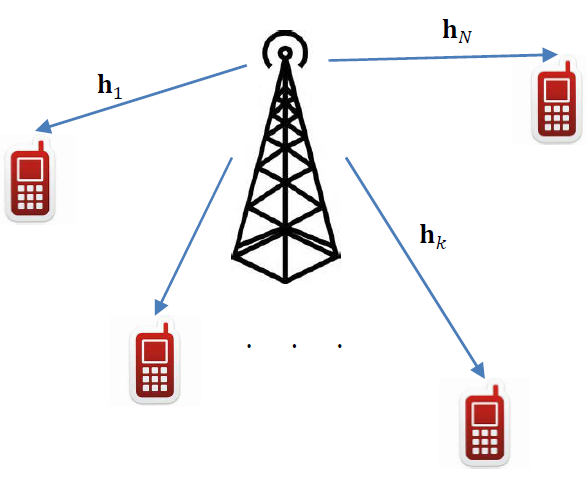
\includegraphics[width=8.7cm]{system.png} % requires the graphicx package
	\caption{Communication scenario}
	\label{fig:system}
\end{figure}
Assuming Alice uses a fixed beamforming strategy, the received signal of Bob $y_b$ is
\begin{eqnarray}
y_b =\mathbf{h}_{0}^{H}\mathbf{w}_0 x_0 + \sum_{i=1}^N \mathbf{h}_{i}^H\mathbf{x}_{i} + n,
\end{eqnarray}
where $x_0$ is the message transmitted from Alice, and $\mathbf{E}\{|x_0|^2\} = 1$; $\mathbf{E}\{\cdot\}$ means expectation; $[\cdot]^H$ denotes hermitian operation. $\mathbf{w}_{0} \in \mathbb{C}^{M \times 1}$  is the beamforming vector of Alice, which satisfies the transmit power constraint $\|\mathbf{w}_0\|_2^2 \leq P_0$. $n \sim \mathcal{N}(0,\sigma_n^2)$ is complex noise. $\mathbf{x}_i \sim \mathcal{N}(\mathbf{0}, \mathbf{Q}_i)$ is the signal transmitted from Helper-$i$. $\mathbf{Q}_i \succeq 0$ is the covariance matrix of signal $\mathbf
{x}_i$. The transmit power constraint of Helper-$i$ is 
\begin{eqnarray}
\mathbf{E}\{\|\mathbf{x}_i\|_2^2\}  = \mathrm{Tr}(\mathbf{E}\{\mathbf{x}_i\mathbf{x}_i^H\} )= \mathrm{Tr}(\mathbf{Q}_i) \leq P_i
\end{eqnarray}
The signal-to-interference-plus-noise ratio of Bob is
\begin{eqnarray} \label{eq:SINR of Bob}
\mathrm{SINR}_b = \frac{\left| \mathbf{h}_{0}^H\mathbf{w}_{0}\right|^2}{\sigma_n^2 + \sum_{i=1}^{N}\mathbf{h}_{i}^H\mathbf{Q}_{i}\mathbf{h}_i}.
\end{eqnarray}

The received signal of Eve $y_e$ is
\begin{eqnarray}
y_e = \mathbf{g}_0^H\mathbf{w}_0x_0 + \sum_{i = 1}^N\mathbf{g}_i^H\mathbf{x}_i + m,
\end{eqnarray}
where $\mathbf{g}_0$ is the $M$ dimensional channel vector from Alice to Eve; $\mathbf{g}_i$ is the $M$ dimensional channel vector from Helper-$i$ to Eve.   Assume $m$ is complex Gaussian such that $m \sim \mathcal{N}(0,\sigma_m^2)$.
The signal-to-interference-plus-noise ratio of the eavesdropper is
\begin{eqnarray}
\mathrm{SINR}_e &=& \frac{\left| \mathbf{g}_{0}^H\mathbf{w}_{0}\right|^2}{\sigma_m^2 + \sum_{i=1}^{N}\mathbf{g}_{i}^H\mathbf{Q}_{i}\mathbf{g}_i} \label{eq:secure_capacity}.
\end{eqnarray}

The achievable secrecy rate at Bob is given by \cite{6728676}
\begin{equation}
R_s = \log_2\left(1 + \mathrm{SINR}_b\right)-\log_2\left(1 + \mathrm{SINR}_e\right).
\end{equation}


\section{Robust Convex Optimization of Secure Communication} \label{sec:robust programming}
%When the eavesdropper is active \cite{gopala2008secrecy,feng_miso}, Alice and the helpers can determine the channels. When the eavesdropper is passive, the channels can be estimated through the local oscillator power inadvertently leaked from the eavesdropper's receiver radio frequency frontend \cite{mukherjee2012detecting,feng_miso}.
In \cite{li_optimal_2011}, the authors address the optimal transmit design for MISO wiretap channel without friendly	 helpers. The non-convex problem is transformed to convex optimization using approximation. The case where only imperfect CSI is available is considered. The methods in \cite{Zhang_Cooperative2015,huang_cooperative_2011} deal with the robust transmission design for MISO wiretap channel. They addressed the problem when there is only one helper to aid the secure transmission. However, normally the channel to the eavesdropper is hard to estimate. When the uncertainty is too great, the guaranteed secrecy rate is too small using the transmit strategy mentioned above. In such scenario, many helpers can cooperatively generate enough artificial noise to guarantee the required secrecy rate.
\subsection{Channel Uncertainty} 
Normally the channels to the eavesdropper are partially known. We assume that  Alice and the helpers have imperfect estimated eavesdropper's channels $\bar{\mathbf{g}}_i$. We define the channel error vectors as
\begin{eqnarray}
\tilde{\mathbf{g}}_i = \mathbf{g}_i-\bar{\mathbf{g}}_i,\forall i = 0,\ldots, N,
\end{eqnarray}
We assume the channel mismatches lie in the bound sets $\mathcal{G}_i=\{\tilde{\mathbf{g}}_i: \tilde{\mathbf{g}}_i^H \mathbf{R}_i\tilde{\mathbf{g}}_i \leq 1\}$ are the channels error vectors;the hermitian positive semi-definite  matrix $\mathbf{R}_i $ defines the variation of channel $\mathbf{g}_i$. 

The helpers use zero forcing (ZF) method to transmit noise to Eve and eliminate interference to Bob.
%The ZF constraint is 
%\begin{eqnarray}
%\mathbf{h}_i^H\mathbf{x}_i =0 , \forall i = 1,\dots, N\label{eq:ZF_constraint}.
%\end{eqnarray}
The ZF constraint can be expressed as
\begin{eqnarray} \label{eq:ZF constraint}
\mathbf{h}_i^H\mathbf{Q}_i \mathbf{h}_i = 0, \forall i = 1,\ldots,N \label{eq:ZF_constraint_relaxed}.
\end{eqnarray}

%\begin{eqnarray}
%&&\mathrm{E}(\|\mathbf{h}_i^H\mathbf{x}_i\|_2^2)\nonumber\\
%&=&\mathrm{E}(\mathbf{h}_i^H\mathbf{x}_i\mathbf{x}_i^H\mathbf{h}_i)\nonumber\\
%&=&\mathbf{h}_i^H\mathbf{Q}_i \mathbf{h}_i = 0, \forall i = 1,\ldots,N \label{eq:ZF_constraint_relaxed}.
%\end{eqnarray}

\subsection{Transmit Strategy of Alice}
The basic idea of the transmit strategy of the system is to let Alice maximize the signal-to-interference-plus-noise ratio of Bob, and leave the job of guaranteeing secure communication to the helpers by generating enough noise to Eve. From \eqref{eq:SINR of Bob} and \eqref{eq:ZF constraint} The signal-to-interference-plus-noise ratio of Bob is 
\begin{eqnarray}
\mathrm{SINR}_b= \frac{\left| \mathbf{h}_{0}^H\mathbf{w}_{0}\right|^2}{\sigma_n^2 }. 
\end{eqnarray}
%$\mathrm{SINR}_b$ is not dependent on the transmit covariance matrices of the helpers. 
The optimal strategy maximizing the signal-to-interference-plus-noise of Alice is maximum ratio transmission (MRT) and the corresponding beamforming vector follows as
\begin{eqnarray}
\mathbf{w}_0 = \sqrt{P_0}\frac{\mathbf{h}_0}{\|\mathbf{h}_0\|_2} \label{eq:optimal_w}.
\end{eqnarray}
%The signal-to-interference-plus-noise ratio of Bob is
%\begin{eqnarray} 
%\mathrm{SINR}_b= \frac{P_0\| \mathbf{h}_{0}\|_2^2}{\sigma_n^2 }.  \label{eq:SINR_b}
%\end{eqnarray}

\subsection{Transmit Strategies of the Helpers}
The signal-to-interference-plus-noise ratio of Eve can be bounded as
\begin{eqnarray}
\mathrm{SINR}_e & < & \frac{\left| \mathbf{g}_{0}^H\mathbf{w}_{0}\right|^2}{\sum_{i=1}^{N}\mathbf{g}_{i}^H\mathbf{Q}_{i}\mathbf{g}_i} \label{eq:neglect_sigma}\\
%&=& \frac{\left|\bar{\mathbf{g}}_0^H\mathbf{w_0} + \tilde{\mathbf{g}}_0^H\mathbf{w}_0\right|^2}{\sum_{i = 1}^N(\bar{\mathbf{g}}+\tilde{\mathbf{g}}_i)^H\mathbf{Q}_i(\bar{\mathbf{g}}+\tilde{\mathbf{g}}_i)}\\
&\leq & \frac{\left|\bar{\mathbf{g}}_0^H\mathbf{w_0}\right|^2 + \left|\tilde{\mathbf{g}}_0^H\mathbf{w}_0\right|^2}{\sum_{i = 1}^N(\bar{\mathbf{g}}+\tilde{\mathbf{g}}_i)^H\mathbf{Q}_i(\bar{\mathbf{g}}+\tilde{\mathbf{g}}_i)}\\
%&\leq & \frac{\left|\bar{\mathbf{g}}_0^H\mathbf{w_0}\right|^2 + \tilde{\mathbf{g}}_0^H\mathbf{w}_0\mathbf{w}_0^H\tilde{\mathbf{g}}_0}{\sum_{i = 1}^N(\bar{\mathbf{g}}+\tilde{\mathbf{g}}_i)^H\mathbf{Q}_i(\bar{\mathbf{g}}+\tilde{\mathbf{g}}_i)}\\
& \leq & \frac{\left|\bar{\mathbf{g}}_0^H\mathbf{w_0}\right|^2 + \max_{\tilde{\mathbf{g}}_i \in \mathcal{G}_i}(\tilde{\mathbf{g}}_0^H\mathbf{w}_0\mathbf{w}_0^H\tilde{\mathbf{g}}_0)}{\sum_{i = 1}^N(\bar{\mathbf{g}}+\tilde{\mathbf{g}}_i)^H\mathbf{Q}_i(\bar{\mathbf{g}}+\tilde{\mathbf{g}}_i)} .
\label{eq:SINR_e}
\end{eqnarray}
In \eqref{eq:neglect_sigma}, the noise is removed. This is because we consider the case where Eve has the best possible receiving performance. 
We want to constrain the maximum signal-to-interference-plus-noise ratio of Eve to a limit. That is 
\begin{eqnarray}
\max \mathrm{SINR}_e \leq \gamma \label{eq:SINR_constraint},
\end{eqnarray} 
where $\gamma$ is the limit. We can guarantee that
\begin{eqnarray}
R_s \geq \log_2\left(1 + P_0\|\mathbf{h}_0\|_2^2/\sigma_n^2\right) - \log_2\left(1 + \gamma\right). \label{eq:secure_capacity1}
\end{eqnarray}
Given the requirement of secrecy rate $R_s$, the predefined limit $\gamma$ can be determined from \eqref{eq:secure_capacity1}.

In order to guarantee the maximum $\mathrm{SINR}_e$ to be within the predetermined limit $\gamma$, the maximum numerator of \eqref{eq:SINR_e} is calculated first by putting \eqref{eq:optimal_w} in \eqref{eq:SINR_e}. We obtain
\begin{equation}
\begin{aligned} \label{eq:numerator problem}
& \underset{\tilde{\mathbf{g}}_{0}}{\text{maximize}}
& & \frac{P_0}{\|\mathbf{h}_0\|_2^2}|\bar{\mathbf{g}}_0^H\mathbf{h}_0|^2 +\frac{P_0}{\|\mathbf{h}_0\|_2^2} \tilde{\mathbf{g}}_0^H\mathbf{h}_0\mathbf{h}_0^H\tilde{\mathbf{g}}_0 \\
& \text{subject to}
& & \tilde{\mathbf{g}}_0^H\mathbf{R}_0\tilde{\mathbf{g}}_0 \leq 1.
\end{aligned}
\end{equation}
Let $\lambda_{\mathrm{max}}(\mathbf{R})$ be the largest eigenvalue of $\mathbf{R}$, then
\begin{eqnarray}
\lambda_{\mathrm{max}}(\mathbf{R})= \max_{\mathbf{y}^H\mathbf{y} \leq 1} \mathbf{y}^H\mathbf{R}\mathbf{y}.
\end{eqnarray}
If we define $\mathbf{R}_0^{1/2}\tilde{\mathbf{g}}_0 = \hat{\mathbf{g}}_0$, problem \eqref{eq:numerator problem} is transformed to the following problem
\begin{equation}
\begin{aligned} \label{eq:numerator problem1}
& \underset{\hat{\mathbf{g}}_{0}}{\text{maximize}}
& & \frac{P_0}{\|\mathbf{h}_0\|_2^2}|\bar{\mathbf{g}}_0^H\mathbf{h}_0|^2 +\frac{P_0}{\|\mathbf{h}_0\|_2^2} \hat{\mathbf{g}}_0^H\mathbf{R}_0^{-1/2}\mathbf{h}_0\mathbf{h}_0^H\mathbf{R}_0^{-1/2}\hat{\mathbf{g}}_0 \\
& \text{subject to}
& & \hat{\mathbf{g}}_0^H\hat{\mathbf{g}}_0 \leq 1.
\end{aligned}
\end{equation}
Then the maximum of \eqref{eq:numerator problem1} is
\begin{eqnarray}
&&\frac{P_0}{\|\mathbf{h}_0\|_2^2}\left(|\bar{\mathbf{g}}_0^H\mathbf{h}_0|^2 + \lambda_{\mathrm{max}}(\mathbf{R}_0^{-1/2}\mathbf{h}_0\mathbf{h}_0^H\mathbf{R}_0^{-1/2})\right)\\
&=&\frac{P_0}{\|\mathbf{h}_0\|_2^2}\left(|\bar{\mathbf{g}}_0^H\mathbf{h}_0|^2 + \|\mathbf{R}_0^{-1/2}\mathbf{h}_0\|_2^2\right)\label{eq:eigen_norm},
\end{eqnarray} 
where \eqref{eq:eigen_norm} follows from the fact that the rank of $\mathbf{R}_0^{-1/2}\mathbf{h}_0$ is 1. Then the constraint of maximum $\mathrm{SINR}_e$ \eqref{eq:SINR_constraint}  becomes
\begin{eqnarray} \label{eq:sum_noise}
\min_{\{\tilde{\mathbf{g}}_i \in \mathcal{G}_i\}}\sum_{i=1}^{N}(\bar{\mathbf{g}}+\tilde{\mathbf{g}}_i)^H\mathbf{Q}_i(\bar{\mathbf{g}}+\tilde{\mathbf{g}}_i) \geq \Gamma  \label{eq:artificial noise constraint},
\end{eqnarray}
where $\Gamma =\frac{P_0\left(|\bar{\mathbf{g}}_0^H\mathbf{h}_0|^2 + \|\mathbf{R}_0^{-1/2}\mathbf{h}_0\|_2^2\right)}{\|\mathbf{h}_0\|_2^2\gamma}$ denotes the total minimum interference needs to be generated by the helpers to the eavesdropper. 

With the goal of minimizing the transmit power of the helpers while guaranteeing the achievable secrecy rate, the problem of secure communication can be formulated as the following problem.

\begin{equation}
\begin{aligned} \label{eq:problem1}
& \underset{\{\mathbf{Q}_i \succeq \mathbf{0}\}}{\text{maximize}}
& & \sum_{i = 1}^{N}\mathrm{Tr}(\mathbf{Q}_i) \\
& \text{subject to}
& & \mathrm{Tr}(\mathbf{Q}_i) \leq P_i, \forall i = 1, \ldots, N\\
&&& \mathbf{h}_i^H \mathbf{Q}_i \mathbf{h}_i= 0, \forall i = 1,\ldots,N\\
&&& \min_{\{\tilde{\mathbf{g}}_i \in \mathcal{G}_i\}}\sum_{i=1}^{N}(\bar{\mathbf{g}}+\tilde{\mathbf{g}}_i)^H\mathbf{Q}_i(\bar{\mathbf{g}}+\tilde{\mathbf{g}}_i) \geq  \Gamma,\\
&&& \forall i = 1, \ldots, N.
\end{aligned}
\end{equation}


Constraint~\eqref{eq:sum_noise} can be decomposed into $N+1$ constraints by introducing the new variables $\tau_i, i =1,\ldots,N$, the physical meaning of which are the minimum interferences that the $N$ helpers need to generate to Eve respectively. The decomposed constraints follow as:
\begin{eqnarray}
&\underset{\tilde{\mathbf{g}}_i \in \mathcal{G}_i }\min(\bar{\mathbf{g}}+\tilde{\mathbf{g}}_i)^H\mathbf{Q}_i(\bar{\mathbf{g}}+\tilde{\mathbf{g}}_i) \geq  \tau_i, \forall i = 1,\ldots,N\label{eq:artificial noise constraint decomposed}\nonumber\\
&\sum_{i =1}^{N}\tau_i \geq \Gamma.
\end{eqnarray}
Then problem \eqref{eq:problem1} can be transformed to the following problem
\begin{equation}
\begin{aligned} \label{eq:problem2}
& \underset{\{\mathbf{Q}_i \succeq \mathbf{0}\},\{\tau_i \geq 0\}}{\text{minimize}}
& & \sum_{i = 1}^{N}\mathrm{Tr}(\mathbf{Q}_i) \\
& \text{subject to}
& & \mathrm{Tr}(\mathbf{Q}_i) \leq P_i, \forall i = 1, \ldots, N\\
&&& \mathbf{h}_i^H \mathbf{Q}_i \mathbf{h}_i= 0, \forall i = 1,\ldots,N\\
&&& \min_{\tilde{\mathbf{g}}_i \in \mathcal{G}_i}(\bar{\mathbf{g}}+\tilde{\mathbf{g}}_i)^H\mathbf{Q}_i(\bar{\mathbf{g}}+\tilde{\mathbf{g}}_i) \geq  \tau_i,\\
&&&\forall i = 1,\ldots,N\\
&&&\sum_{i =1}^{N}\tau_i \geq \Gamma.
\end{aligned}
\end{equation}

%The implication of \eqref{eq:artificial noise constraint decomposed} is
%\begin{eqnarray}
%\tilde{\mathbf{g}}_i^H\mathbf{R}_i\tilde{\mathbf{g}} _i - 1\leq 0  \Rightarrow (\bar{\mathbf{g}}_i+\tilde{\mathbf{g}}_i)^H\mathbf{Q}_i(\bar{\mathbf{g}}_i+\tilde{\mathbf{g}}_i) - \tau_i \geq 0.
%\end{eqnarray}
According to the S-Procedure \cite{ConvexOpt_Boyd}, Constraint \eqref{eq:artificial noise constraint decomposed}  in the linear matrix inequality (LMI) form is
\begin{eqnarray}
\left[ {\begin{array}{cc}
	\lambda_i\mathbf{R}_i+\mathbf{Q}_i  & \mathbf{Q}_i\bar{\mathbf{g}}_i \\
	\bar{\mathbf{g}}_i^H\mathbf{Q}_i& \bar{\mathbf{g}}_i^H\mathbf{Q}_i\bar{\mathbf{g}} _i- \tau_i -\lambda_i\\
	\end{array} } \right] \succeq \mathbf{0},
\end{eqnarray}
where $\lambda_i \geq 0$ is a new variable introduced by S-procedure. Then Problem \eqref{eq:problem2} can be solved using convex optimization tools such as CVX\cite{cvx}.

%So problem \eqref{eq:problem2} can be transformed to the following problem
%\begin{equation}
%\begin{aligned} \label{eq:problem3}
%& \underset{\{\mathbf{Q}_i\},\{\lambda_i\},\{\tau_i\}}{\text{maximize}}
%& & \sum_{i = 1}^{N}\mathrm{Tr}(\mathbf{Q}_i) \\
%& \text{subject to}
%& & \mathrm{Tr}(\mathbf{Q}_i) \leq P_i, \forall i = 1, \ldots, N\\
%&&& \mathbf{h}_i^H \mathbf{Q}_i \mathbf{h}_i= 0, \forall i = 1,\ldots,N\\
%&&& \left[ {\begin{array}{cc}
%	\lambda_i\mathbf{R}_i+\mathbf{Q}_i  & \mathbf{Q}_i\bar{\mathbf{g}}_i \\
%	\bar{\mathbf{g}}_i^H\mathbf{Q}_i & \bar{\mathbf{g}}_i^H\mathbf{Q}_i\bar{\mathbf{g}}_i - \tau_i -\lambda_i
%	\end{array} } \right] \succeq \mathbf{0},\\
%&&& \forall i = 1, \ldots, N\\
%&&&\sum_{i =1}^{N}\tau_i \geq \Gamma.
%\end{aligned}
%\end{equation}
%
%Problem \eqref{eq:problem2} and \eqref{eq:problem3} are equivalent. By solving problem \eqref{eq:problem3} using convex optimization tools such as CVX\cite{cvx}, we can solve the secure communication problem.

%Based on the solved covariance matrices,  $M$ dimensional noise $\mathbf{x}_i$ can be generated and sent out by Jammer-$i$. The transmitted signal of Jammer-$i$ is 
%\begin{eqnarray}
%\mathbf{x}_i = \mathbf{Q}_i^{1/2}\mathbf{r}_i.
%\end{eqnarray} 
%$\mathbf{r}_i = [r_{i1},\ldots,r_{iM}]^T$ is Gaussian noise such that $\mathbf{r}_i \sim \mathcal{N}(\mathbf{0},\mathbf{I})$, where $[\cdot]^T$ means transpose operation, and $\mathbf{I}$ is an $M \times M$ identity matrix. 
%The block diagram of the transmitter of Jammer-$i$ is shown in Fig.~\ref{fig:transmitter}, where the random noise generators generate independent noise waveforms.
%\begin{figure}[h]
%	\centering
%	\includegraphics[width=8.8cm]{transmitter.pdf} % requires the graphicx package
%	\caption{Block diagram of the transmitter of Jammer-$i$}
%	\label{fig:transmitter}
%\end{figure}

\section{Distributed algorithm} \label{sec:distributed algorithm}
Solving problem \eqref{eq:problem2} requires a central unit to collect all the channel information and calculate the covariance matrices of all the helpers. When the number of helpers increases, the centralized algorithm dose not scale well. 
In this section, we analyze the structure of the problem and propose a distributed algorithm. 

\emph{Proposition 1:} $\{\tau_i^*\}, \{\mathbf{Q}_i^*\}, i = 1, \ldots, N$ are the solution of problem \eqref{eq:problem2}. If $\tau_k^* > 0$ and
\begin{eqnarray}
\frac{\tau_j^*}{\mathrm{Tr}(\mathbf{Q}_j^*)} > \frac{\tau_k^*}{\mathrm{Tr}(\mathbf{Q}_k^*)} \label{eq:efficiency},
\end{eqnarray}
then $\mathrm{Tr}(\mathbf{Q}_j^*) = P_j$.

\emph{Proof:} Assuming $\mathrm{Tr}(\mathbf{Q}_j^*) < P_j$, we construct $\tilde{\mathbf{Q}}_j = (1 + \delta) \mathbf{Q}_j^*$ such that $\mathrm{Tr}(\tilde{\mathbf{Q}}_j) = P_j$ and $\tilde{\mathbf{Q}}_k = \frac{\tau_k^* - \delta\tau_j^*}{\tau_k^*} \mathbf{Q}_k^*$. We have
\begin{eqnarray}
\min_{\tilde{\mathbf{g}}_j \in \mathcal{G}_j}(\bar{\mathbf{g}}_j+\tilde{\mathbf{g}}_j)^H\tilde{\mathbf{Q}}_j(\bar{\mathbf{g}}_j+\tilde{\mathbf{g}}_j)\geq (1+ \delta)\tau_j^*,\\
\min_{\tilde{\mathbf{g}}_k \in \mathcal{G}_k}(\bar{\mathbf{g}}_k+\tilde{\mathbf{g}}_k)^H\tilde{\mathbf{Q}}_k(\bar{\mathbf{g}}_k+\tilde{\mathbf{g}}_k) \geq \tau_k^* - \delta\tau_j^*.
\end{eqnarray}
%The same amount interference generated by Jammer-$k$ and Jammer-$j$ to Eve can be guaranteed
%\begin{eqnarray}
%&&(\bar{\mathbf{g}}_j+\tilde{\mathbf{g}}_j)^H\tilde{\mathbf{Q}}_j(\bar{\mathbf{g}}_j+\tilde{\mathbf{g}}_j) \nonumber+ (\bar{\mathbf{g}}_k+\tilde{\mathbf{g}}_k)^H\tilde{\mathbf{Q}}_k(\bar{\mathbf{g}}_k+\tilde{\mathbf{g}}_k)\nonumber\\
%&\geq&  \tau_k^* + \tau_j^*.
%\end{eqnarray}
It is obvious that $\tilde{\mathbf{Q}}_k, \tilde{\mathbf{Q}}_j$ and other $\mathbf{Q}_i^*, i \neq k,j$ satisfy constraint \eqref{eq:sum_noise}. But
\begin{eqnarray}
&&\mathrm{Tr}(\tilde{\mathbf{Q}}_k) + \mathrm{Tr}(\tilde{\mathbf{Q}}_j)\\
%&=&\frac{\tau_k^* - \delta\tau_j^*}{\tau_k^*} \mathrm{Tr}(\mathbf{Q}_k^*)  + (1 + \delta)\mathrm{Tr}(\mathbf{Q}_j^*)\\
&=&\mathrm{Tr}(\mathbf{Q}_k^*) + \mathrm{Tr}(\mathbf{Q}_j^*) + \frac{\delta\tau_k^*\mathrm{Tr}(\mathbf{Q}_j^*)-\delta\tau_j^*\mathrm{Tr}(\mathbf{Q}_k^*)}{\tau_k^*}\\
&<&\mathrm{Tr}(\mathbf{Q}_k^*) + \mathrm{Tr}(\mathbf{Q}_j^*), \label{eq:contradiction}
\end{eqnarray}
where \eqref{eq:contradiction} comes from  \eqref{eq:efficiency}.
Inequality \eqref{eq:contradiction} means $\tilde{\mathbf{Q}}_k, \tilde{\mathbf{Q}}_j$ and other $\mathbf{Q}_i^*, i \neq k,j$ are a better solution of problem \eqref{eq:problem2}, which is a contradiction.$\blacksquare$

The term $\frac{\tau_i*}{\mathrm{Tr}(\mathbf{Q}_i^*)}$ defines the interference generated per unit power by Helper-$i$. We call it the transmit efficiency of Helper-$i$. Proposition 1 shows the fact that in order to generate the interference to the eavesdropper in the most efficient way, the helpers with higher transmit efficiency should transmit artificial noise as much as possible.

\emph{Proposition 2:} $\{\tau_i^*\}, \{\mathbf{Q}_i^*\}, i = 1, \ldots, N$ are the solution of problem \eqref{eq:problem2}. For any $ \tau'_i > 0$ such that problem \eqref{eq:same_efficiency} is feasible, $ \mathbf{Q}'_i$ is the solution of problem \eqref{eq:same_efficiency}. If $\tau_i^* > 0$, $\frac{\tau_i^*}{\text{Tr}(\mathbf{Q}_i^*)} = \frac{\tau'_i}{\text{Tr}(\mathbf{Q}'_i)}$.
\begin{eqnarray}\label{eq:same_efficiency}
\begin{aligned} 
& \underset{\mathbf{Q}_i \succeq \mathbf{0}}{\text{minimize}}
& & \text{Tr}(\mathbf{Q}_i)\\
& \text{subject to}
& & \min_{\tilde{\mathbf{g}}_i \in \mathcal{G}_i}(\bar{\mathbf{g}}+\tilde{\mathbf{g}}_i)^H\mathbf{Q}_i(\bar{\mathbf{g}}+\tilde{\mathbf{g}}_i) \geq \tau'_i,\\
&&& \text{Tr}\left(\mathbf{Q}_i\right) \leq P_i,\\ 
&&&\text{Tr}\left(\mathbf{h}_i^H\mathbf{Q}_i\mathbf{h}_i\right) = 0.
\end{aligned}
\end{eqnarray}

\emph{Proof:} If $\frac{\tau_i^*}{\text{Tr}(\mathbf{Q}_i^*)} > \frac{\tau'_i}{\text{Tr}(\mathbf{Q}'_i)}$, let $\tilde{\mathbf{Q}}_i = \delta\mathbf{Q}_i^ *$ such that $\delta\tau_i^* = \tau'_i$. Then $\text{Tr}(\tilde{\mathbf{Q}}_i) < \text{Tr}(\mathbf{Q}'_i)$. $\tilde{\mathbf{Q}}_i$ satisfies all the constraints of problem \eqref{eq:same_efficiency}. $\tilde{\mathbf{Q}}_i$  is a better solution of problem \eqref{eq:same_efficiency} , which is a contradiction.

If $\frac{\tau_i^*}{\text{Tr}(\mathbf{Q}_i^*)} < \frac{\tau'_i}{\text{Tr}(\mathbf{Q}'_i)}$, we let $\tilde{\mathbf{Q}}_i = \delta\mathbf{Q}'_i$ such that $\delta\tau'_i = \tau_i^*$. Then $\text{Tr}(\tilde{\mathbf{Q}}_i) < \text{Tr}(\mathbf{Q}^*_i)$. So,  $\tilde{\mathbf{Q}}_i$ and other $\mathbf{Q}_k^*, k \neq i$ are a better solution of problem \eqref{eq:problem2}, which is a contradiction.$\blacksquare$

Proposition 2 describes the fact that the transmit efficiency of problem \eqref{eq:problem2} can be obtained by solving problem \eqref{eq:same_efficiency}.

Proposition 2 can be interpreted using Fig.~\ref{fig:interpretation of subproblems}. Ellipsoid B represents the uncertainty of the eavesdropper's channel. When $\mathbf{g}_i$ is in ellipsoid A, we have $\mathbf{g}_i^H\mathbf{Q}_i\mathbf{g}_i \leq  \tau_{i}$. We want to find the ``biggest" ellipsoid A constrained by the power constraint and ZF constraint, such that ellipsoid B is completely outside of the ellipsoid A. Here the ``biggest" ellipsoid corresponds to the $\mathbf{Q}_i$ which has the smallest sum of eigenvalues.  From the figure, we can tell that the shape of ellipsoid A is unchanged, but $\mathbf{Q}_i$ scales with $\tau_i$.
\begin{figure}[ht]
	\centering
	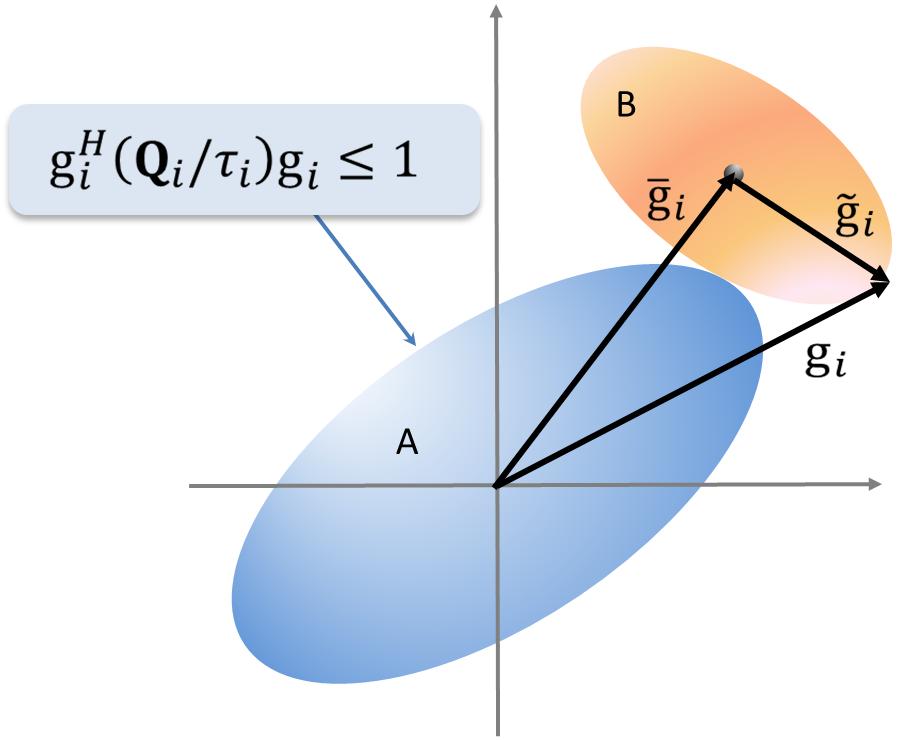
\includegraphics[width=8.8cm]{subproblem.pdf} % requires the graphicx package
	\caption{Interpretation of problem \eqref{eq:subproblem1}}
	\label{fig:interpretation of subproblems}
\end{figure}
Considering the case where  ellipsoid B is enlarged such that it includes the origin, then we cannot find $\mathbf{Q}_i$ to exclude ellipsoid B outside ellipsoid A when $\tau_i$ is positive. That means, if  $\bar{\mathbf{g}}_i^H\mathbf{R}_i\bar{\mathbf{g}}_i \leq 1, \forall i = 1, \ldots,N$, positive interference generated to the eavesdropper cannot be guaranteed, and positive secrecy rate cannot be guaranteed no matter how large the transmit power of the helpers have.   


%Proposition 2 describes the fact that no matter how much interference is needed to be transmitted by each helper, the transmit efficiency remains the same. 

\emph{Proposition 3:} If problem \eqref{eq:same_efficiency} is feasible, there is a solution $\mathbf{Q}_i^*$, the rank of which is $1$.

\emph{Proof :} Let $\mathbf{P}_{\perp}$ denote the orthogonal complement projector of $\mathbf{h}_0$. Let $\mathbf{P}_{\perp}\tilde{\mathbf{x}}_i = \mathbf{x}_i$, $\mathbf{X}_i = \mathbf{E}\{\tilde{\mathbf{x}}_i\tilde{\mathbf{x}}_i^H\}$ Then problem \eqref{eq:same_efficiency} is equivalent to 
\begin{align} 
& \underset{\mathbf{X}_i \succeq \mathbf{0}}{\text{minimize}}
& & \text{Tr}(\mathbf{X}_i)\\
& \text{subject to}
& & \min_{\tilde{\mathbf{g}}_i \in \mathcal{G}_i}(\bar{\mathbf{g}}+\tilde{\mathbf{g}}_i)^H\mathbf{P}_{\perp}\mathbf{X}_i\mathbf{P}_{\perp }^H(\bar{\mathbf{g}}+\tilde{\mathbf{g}}_i) \geq \tau'_i, \label{eq:interference_budget}\\
&&& \text{Tr}\left(\mathbf{X}_i\right) \leq P_i.\label{eq:power}\\ 
\end{align}
Let $\lambda^*$ be an optimal dual variable for the constraint \eqref{eq:power}, $\mathbf{\Phi}^* \succeq \mathbf{0}$
be that for the constraint \eqref{eq:interference_budget}, and $\mathbf{\Psi}^*$ be that for the constraint $\mathbf{X}_i \succeq \mathbf{0}$. The KKT conditions related to $\mathbf{X}_i^*$ are 
\begin{eqnarray}
	\mathbf{\Psi}^*=\mathbf{I} - (\bar{\mathbf{g}}_i + \tilde{\mathbf{g}}_i^*)\mathbf{P}_{\perp}\mathbf{\Phi}^*\mathbf{P}_{\perp}^H(\bar{\mathbf{g}}_i + \tilde{\mathbf{g}}_i^*)^H + \lambda^*\mathbf{I} \label{eq:rank_n-1}\\
	\mathbf{\Psi}^*\mathbf{X}_i^* = 0 \label{eq:nullity} 
\end{eqnarray}
In \eqref{eq:rank_n-1}, $\tilde{\mathbf{g}}_i^*$ means the worst-case channel mismatch for $\mathbf{X}_i^*$. 

Equation \eqref{eq:nullity} implies that columns of $\mathbf{X}_i^*$ must lie in the nullspace of $\mathbf{\Psi}^*$. Therefore
\begin{eqnarray} 
\text{rank}\left(\mathbf{X}_i^*\right) \leq \text{Nullity}\left(\mathbf{\Psi}^*\right) \leq N - \text{rank}\left(\mathbf{\Psi}^*\right) \label{eq:KKT_rank}
\end{eqnarray}
Let $\mathbf{f}_i = (\bar{\mathbf{g}}_i + \tilde{\mathbf{g}}_i^*)\left(\mathbf{P}_{\perp}\mathbf{\Phi}^*\mathbf{P}_{\perp}^H\right)^{1/2}$
From \eqref{eq:rank_n-1}
\begin{eqnarray}
\text{rank}\left(\mathbf{\Psi}^*\right) = \text{rank}\left((1 + \lambda^*)\mathbf{I} - \mathbf{f}_i\mathbf{f}_i^H\right)
\end{eqnarray}
$\text{rank}\left((1 + \lambda^*)\mathbf{I} - \mathbf{f}_i\mathbf{f}_i^H\right)$ due to the matrix sturcture. Then we have $\text{rank}\left(\mathbf{\Psi}^*\right) \geq N - 1$. From \eqref{eq:KKT_rank}, we get $\text{rank}\left(\mathbf{X}_i^*\right) = 1$. Because $\mathbf{Q}_i = \mathbf{P}_{\perp}\mathbf{X}_i\mathbf{P}_{\perp}^H$, $\text{rank}\left(\mathbf{Q}_i^*\right) = 1$.$\blacksquare$

Let $\bar{\mathbf{p}}_i = \mathbf{P}_{\perp}\bar{\mathbf{g}}_i$, $\tilde{\mathbf{p}}_i = \mathbf{P}_{\perp}\tilde{\mathbf{g}}_i$, $\mathcal{P}_i = \{\tilde{\mathbf{p}}_i:\tilde{\mathbf{p}}_i^H\mathbf{P}_{\perp}\mathbf{R}_i\mathbf{P}_{\perp}\tilde{\mathbf{p}}_i \leq 1 \}$. From Proposition 3, problem \eqref{eq:same_efficiency} can be simplified as the following problem
\begin{eqnarray}
\begin{aligned}  \label{eq:same_efficiency_vector}
& \underset{\mathbf{w}_i}{\text{minimize}}
& & \|\mathbf{w}_i\|^2\\
& \text{subject to}
& & \min_{\tilde{\mathbf{g}}_i \in \mathcal{G}_i}\|(\bar{\mathbf{p}}+\tilde{\mathbf{p}}_i)^H\mathbf{w}_i\|^2 \geq \tau'_i, \label{eq:interference_budget}\\
&&& \|\mathbf{w}_i\|_2^2 \leq P_i.\label{eq:power}\\ 
\end{aligned}
\end{eqnarray}
where $\mathbf{w}_i\mathbf{w}_i^H = \mathbf{X}_i$; $\|\cdot\|$ denotes euclidean norm.

\emph{Lemma 1:} The solution $\mathbf{w}_i^*$ must have the following form 
\begin{equation}
\mathbf{w}_i^* = \alpha (\bar{\mathbf{p}}
_i+\tilde{\mathbf{p}}_i^*)
\end{equation}
where $\alpha > 0$; $\tilde{\mathbf{p}}_i^*$ is the worst-case vector such that $\|(\bar{\mathbf{p}}+\tilde{\mathbf{p}}_i^*)\mathbf{w}_i^*\|^2 \geq \tau'_i$

\emph{Proof ;} Assuming $\mathbf{w}_i^* \neq \alpha (\bar{\mathbf{p}}
_i+\tilde{\mathbf{p}}_i^*), \forall \alpha > 0$. We construct a vector $\mathbf{w}'_i = \alpha (\bar{\mathbf{p}}
_i+\tilde{\mathbf{p}}_i^*)$, such that $\|\mathbf{w}_i^*\| =\|\mathbf{w}'_i\|$ According to Cauchy-Schwarz inequality, 
\begin{eqnarray}
\|(\bar{\mathbf{p}}
_i+\tilde{\mathbf{p}}_i^*)\mathbf{w}_i^*\|^2 < \|(\bar{\mathbf{p}}
_i+\tilde{\mathbf{p}}_i^*)\|^2\|\mathbf{w}_i^*\|^2 \leq \|(\bar{\mathbf{p}}
_i+\tilde{\mathbf{p}}_i^*)\|^2\|\mathbf{w}'_i\|^2
\end{eqnarray}
Let $\delta \in (0,1)$, such that $\|(\bar{\mathbf{p}}
_i+\tilde{\mathbf{p}}_i)\|^2\|\mathbf{w}'_i\|^2 = \tau'_i$. It is obvious that $\delta\mathbf{w}'_i$ is a better solution, which is a contradiction. $\blacksquare$


Based on Proposition 1 and Proposition 2, we propose the following algorithm.




\begin{algorithm}
	\caption{}\label{alg:distributed}
	\begin{algorithmic}
		\item[0.] Set $\tau'_i$ to a small value. 
		\item[1.] Solve \eqref{eq:same_efficiency} for each helper to get $\mathbf{Q}_i$, and calculate the transmit efficiency $\varepsilon_i = \frac{\tau'_i}{\mathrm{Tr}(\mathbf{Q}_i)}$. If \eqref{eq:same_efficiency} is infeasible, set $\varepsilon_i = 0$.
		\item[2.] Broadcast $\varepsilon_i$ and $P_i$ to other helpers. 
		\item[3.] For each helper set $\mathcal{E} =\{ {\varepsilon_i,\ldots, \varepsilon_N}\}$ and $\mathcal{I} =\{\}$.
		\item[4.] For each helper find the maximum transmit efficiency in set $\mathcal{E}$, that is $\varepsilon_i = \max~\mathcal{E}$ (if $\mathcal{E}$ is empty,  the maximum transmit efficiency returned is 0). If $\varepsilon_i = 0$, goto step 6; else $\mathcal{I} := \mathcal{I} + \{i\}$; $\mathcal{E} := \mathcal{E}  - \{\varepsilon_i\}$.
		\item[5.] If $\Gamma \geq \varepsilon_{i} P_i$, $\mathbf{Q}_{i}^* = \frac{P_i}{\mathrm{Tr(\mathrm{Q}}_i)}\mathbf{Q}_i$, $\Gamma := \Gamma - \varepsilon_iP_i$, goto step 4; else $\mathbf{Q}_{i}^* = \frac{\Gamma}{\tau'_i}\mathbf{Q}_i$, go to step 7.
		\item[6.] The required secrecy rate cannot be guaranteed.
		\item[7.] If $i \in \mathcal{I}$, the transmit covariance of Helper-$i$ is $\mathbf{Q}_i^*$, otherwise the transmit covariance is $\mathbf{0}$.
		
	\end{algorithmic}
\end{algorithm}

The basic idea of Algorithm \ref{alg:distributed} is that each helper calculates the transmit efficiency of generating interference to the eavesdropper and the algorithm always chooses the most efficient helper to generate as much interference as possible. In the algorithm, each helper solves a convex optimization problem only once distributively, and broadcasts the scalar transmit efficiency and transmit power limit to other helpers. 


\section{Numerical Results} \label{sec:numerical results}
The radio network in Fig.~\ref{fig:system} was simulated. Alice and the helpers have four transmit antennas each. The channel from Alice to Bob is randomly selected and normalized. The channels from the helpers to Bob and from the transmitters to Eve are randomly generated such that $\|\mathbf{h}_i\| = \alpha$ and $\|\bar{\mathbf{g}}_i\| = \beta$. $\alpha,\beta\in  [0.1,10]$ are independent uniformly distributed random variables, which is used to simulate the random distance from the transmitters to Bob and Eve. 
Positive hermitian matrix $\mathbf{R}_i$ is randomly generated, and $\|\mathbf{R}_i\|_F = s$. Simulation parameter $s$ defines the size of the eavesdropper's channel uncertainty. The larger $s$ is, the smaller the channel uncertainty is. 
For simplicity, we assume Alice and all the helpers have the same transmit power. That is $P_0=P_i = P$. 
The noise variance of Bob is normalized to 1. We set $\mathrm{SNR}_b = 20 \mathrm{dB}$, which means $P = 100$.


\begin{figure}[!ht]
	\centering
	\includegraphics[width=8.8cm]{Changing_Cs.eps} % requires the graphicx package
	\caption{Relationship of total transmit power with required secrecy rates.}
	\label{fig:Changing_Cs}
\end{figure}

Fig.~\ref{fig:Changing_Cs} shows the relationship between the total transmit power and the required achievable secrecy rate. Simulation parameter is set $s = 1$. When there are more helpers, the total transmit power is lower. It is because that there are more strategies for the helpers to choose to generate noise. When the requirement of achievable secrecy rate is higher, more total transmit power is needed to generate enough noise to confuse the eavesdropper. In the simulation, compared to the transmit power limit of each helper, the actual total transmit power of the helpers is small. It means on average, the helpers only need small transmit power to generate noise to the eavesdropper.

\begin{figure}[!ht]
	\centering
	\includegraphics[width=8.8cm]{Changing_s.eps} % requires the graphicx package
	\caption{Relationship of total transmit power with the simulation parameter $s$.}
	\label{fig:Changing_s}
\end{figure}

Fig.~\ref{fig:Changing_s} shows  the relationship between the total transmit power and the simulation parameter $s$. In this simulation, we fix the secrecy rate requirement $R_s \geq 3 $ b/s/Hz. When $s$ is small, which means the uncertainty is large, the helpers need more power to transmit noise to realize the required secure communication. This is because when the uncertainty is larger, the helpers need to transmit more noise to make sure that the performance of the eavesdropper can be degraded enough to guarantee the achievable secrecy rate for all the possible eavesdropper's channels.

\begin{figure}[!ht]
	\centering
	\includegraphics[width=8.8cm]{Cs_success.eps} % requires the graphicx package
	\caption{Relationship of successfully realizing secure communication with required secrecy rates.}
	\label{fig:Cs_success}
\end{figure}
\begin{figure}[!ht]
	\centering
	\includegraphics[width=8.8cm]{s_success.eps} % requires the graphicx package
	\caption{Relationship of successfully realizing secure communication with the simulation parameter $s$.}
	\label{fig:s_success}
\end{figure}

All the helpers may still not be able to generate enough noise to realize required secrecy rate. Fig.~\ref{fig:Cs_success} and Fig.~\ref{fig:s_success} show the relationship of successfully realizing the required secure communication with the secrecy rate requirement and the eavesdropper's channel uncertainty. For Fig.~\ref{fig:Cs_success}, we fix the simulation parameter $s = 1$. For Fig.~\ref{fig:s_success} we fix the required secrecy rate $R_s \geq 3$ b/s/Hz. It can be shown that higher secrecy rate requirement and larger channel uncertainty will cause less success rate of the required secure communication. But by increasing the number of helpers and using the distributed algorithm proposed in Section \ref{sec:distributed algorithm} which scales well with a large number of helpers, we can increase the success rate of secure communication easily. 

% An example of a floating figure using the graphicx package.
% Note that \label must occur AFTER (or within) \caption.
% For figures, \caption should occur after the \includegraphics.
% Note that IEEEtran v1.7 and later has special internal code that
% is designed to preserve the operation of \label within \caption
% even when the captionsoff option is in effect. However, because
% of issues like this, it may be the safest practice to put all your
% \label just after \caption rather than within \caption{}.
%
% Reminder: the "draftcls" or "draftclsnofoot", not "draft", class
% option should be used if it is desired that the figures are to be
% displayed while in draft mode.
%
%\begin{figure}[!t]
%\centering
%\includegraphics[width=2.5in]{myfigure}
% where an .eps filename suffix will be assumed under latex, 
% and a .pdf suffix will be assumed for pdflatex; or what has been declared
% via \DeclareGraphicsExtensions.
%\caption{Simulation results for the network.}
%\label{fig_sim}
%\end{figure}

% Note that IEEE typically puts floats only at the top, even when this
% results in a large percentage of a column being occupied by floats.


% An example of a double column floating figure using two subfigures.
% (The subfig.sty package must be loaded for this to work.)
% The subfigure \label commands are set within each subfloat command,
% and the \label for the overall figure must come after \caption.
% \hfil is used as a separator to get equal spacing.
% Watch out that the combined width of all the subfigures on a 
% line do not exceed the text width or a line break will occur.
%
%\begin{figure*}[!t]
%\centering
%\subfloat[Case I]{\includegraphics[width=2.5in]{box}%
%\label{fig_first_case}}
%\hfil
%\subfloat[Case II]{\includegraphics[width=2.5in]{box}%
%\label{fig_second_case}}
%\caption{Simulation results for the network.}
%\label{fig_sim}
%\end{figure*}
%
% Note that often IEEE papers with subfigures do not employ subfigure
% captions (using the optional argument to \subfloat[]), but instead will
% reference/describe all of them (a), (b), etc., within the main caption.
% Be aware that for subfig.sty to generate the (a), (b), etc., subfigure
% labels, the optional argument to \subfloat must be present. If a
% subcaption is not desired, just leave its contents blank,
% e.g., \subfloat[].


% An example of a floating table. Note that, for IEEE style tables, the
% \caption command should come BEFORE the table and, given that table
% captions serve much like titles, are usually capitalized except for words
% such as a, an, and, as, at, but, by, for, in, nor, of, on, or, the, to
% and up, which are usually not capitalized unless they are the first or
% last word of the caption. Table text will default to \footnotesize as
% IEEE normally uses this smaller font for tables.
% The \label must come after \caption as always.
%
%\begin{table}[!t]
%% increase table row spacing, adjust to taste
%\renewcommand{\arraystretch}{1.3}
% if using array.sty, it might be a good idea to tweak the value of
% \extrarowheight as needed to properly center the text within the cells
%\caption{An Example of a Table}
%\label{table_example}
%\centering
%% Some packages, such as MDW tools, offer better commands for making tables
%% than the plain LaTeX2e tabular which is used here.
%\begin{tabular}{|c||c|}
%\hline
%One & Two\\
%\hline
%Three & Four\\
%\hline
%\end{tabular}
%\end{table}


% Note that the IEEE does not put floats in the very first column
% - or typically anywhere on the first page for that matter. Also,
% in-text middle ("here") positioning is typically not used, but it
% is allowed and encouraged for Computer Society conferences (but
% not Computer Society journals). Most IEEE journals/conferences use
% top floats exclusively. 
% Note that, LaTeX2e, unlike IEEE journals/conferences, places
% footnotes above bottom floats. This can be corrected via the
% \fnbelowfloat command of the stfloats package.




\section{Conclusion} \label{sec:conclusion}
This paper discusses a method to implement secure communication. The channels from the intended transmitter and the helpers to the intended receiver are known. But the channels to the eavesdropper are imperfectly known. The intended transmitter uses MRT to maximize the signal-to-interference-plus-noise ratio of the intended receiver. The helpers transmit noise to degrade the performance of the eavesdropper to guarantee the required secrecy rate. The structure of the transmitted noise is exploited and the transmit strategies of the helpers are formulated as a robust convex optimization problem, in which the transmit covariance matrices are the optimization variables. Based on the solved transmit covariances of the helpers, the required secure communication can be implemented. In order to ease the implementation of secure communication, a distributed algorithm, which scales well with a large number of helpers, is proposed. Simulation results show that with the aid of the helpers, robust secure communication can be realized.




% conference papers do not normally have an appendix


% use section* for acknowledgment
%\section*{Acknowledgment}


%The authors would like to thank...





% trigger a \newpage just before the given reference
% number - used to balance the columns on the last page
% adjust value as needed - may need to be readjusted if
% the document is modified later
%\IEEEtriggeratref{8}
% The "triggered" command can be changed if desired:
%\IEEEtriggercmd{\enlargethispage{-5in}}

% references section

% can use a bibliography generated by BibTeX as a .bbl file
% BibTeX documentation can be easily obtained at:
% http://www.ctan.org/tex-archive/biblio/bibtex/contrib/doc/
% The IEEEtran BibTeX style support page is at:
% http://www.michaelshell.org/tex/ieeetran/bibtex/
%\bibliographystyle{IEEEtran}
% argument is your BibTeX string definitions and bibliography database(s)
%\bibliography{IEEEabrv,../bib/paper}
%
% <OR> manually copy in the resultant .bbl file
% set second argument of \begin to the number of references
% (used to reserve space for the reference number labels box)
%\begin{thebibliography}{1}
\bibliographystyle{IEEEtran}
\bibliography{IEEEabrv,PHY}
%\end{thebibliography}




% that's all folks
\end{document}


